\chapter{Introduction}
\label{ch:Introduction}
Answer Set Programming (ASP) is one of the most successful programming paradigms for declarative problem solving in particular in the field of knowledge representation and reasoning. As such, it has found applications in many different fields both in academic and industry work~\cite{EGL16}.
However, even though it has been around for over 20 years~\cite{Nie99, MT98}, there is still a significant lack of good workflow tools. Tools like a testing suite, debugging tool or a annotation language can help make the development process more streamlined and allow different approaches that have proven very effective in conventional programming languages such as test driven development (TDD,~\cite{Fra+03}). Research into these topics exists and has yielded results, however many topics remain unexplored.

This thesis will focus on one of these mostly unexplored topics which is code coverage for ASP. Code coverage is a concept that is widely used in conventional programming languages. It's efficacy has been evaluated many times and it has proven to be one of the most practical ways to test the adequacy of existing test suites or to generate new test suites with high fault detection~\cite{GJG14}.
Unfortunately, the coverage concepts applied in conventional testing cannot be easily applied to answer set programs. Notions such as \emph{path coverage} or \emph{branch coverage} common in procedural programming languages rely on evaluating paths through the control flow graph of a program, but such a graph cannot be constructed for answer set programs since, due to their declarative nature, no explicit notion of execution exists.

Testing and coverage has been discussed for declarative programming. In~\cite{BJ98} \citeauthor{BJ98} introduce coverage notions for logic programs based on the Prolog model of posing queries to a program and resolving them using SLD resolution. The concepts of unification and anti-instances are used to define the coverage metrics. This means that even though Prolog is a declarative language and in many ways similar to ASP, these notions are not compatible with ASP as it relies on rule instantiation instead of unification.
Work has also been done on testing constraint programs, another paradigm used in logic programming, however it was concluded, that developing notions of test coverage would not be possible in this case~\cite{LGL10}.

Finally, while general approaches to testing in ASP have been discussed multiple times~\cite[examples:][]{GOT17, ABR21, Oet22}, the only attempt at realising code coverage for answer set programs has been done in the paper \citetitle{Jan+10} by~\textcite{Jan+10}. 
There, five coverage metrics are defined for propositional normal programs based on the existing concepts of path and branch coverage in conventional testing. The contributions of this work to this topic are twofold:
\begin{enumerate}
    \item Introduction of a syntactic transformation of answer set programs which allows the computation of the coverage metrics defined by \citeauthor{Jan+10} using the integrated ASP system clingo.
    \item Extension of the given definitions so that they can also apply to more complex program classes.
\end{enumerate}

\begin{comment}
- Answer Set Programming is of growing importance in both academic and industry work (source?) and clingo is a popular solver for this

- Workflow Tools that make working with such programs easier and more comfortable barely exist. Research into these topics is only 
now getting more traction (source?)

- Testing is a very important part of a conventional software design approach.(source?)

- The topic of code coverage and it's use for conventional programming languages has been shown (source?)

- With this work I want to build on the previous work done on code coverage in answer set programming in this paper by~\textcite{Jan+10}

- To this end I developed a way to efficiently implement the coverage metrics defined in the paper.

- My implementation allows me to compute coverage using answer set programming. It also extends the given metrics to function with
almost all existing language construct instead of just for propositional programs.
\end{comment}

%%%%%%%%%%%%%%%%%%%%%%%%%%%%%%%%%%%%%%%%%%%%%%%%%%%%%%%%%%%%%%%%

\chapter{Preliminaries on answer set programming}
\label{ch:Preliminaries on answer set programming}
This chapter will provide a short introduction to ASP and lay down the basic definitions that will be used in the rest of the thesis. As mentioned in \Cref{ch:Introduction}, the coverage metrics are restricted to propositional normal programs. Hence we will focus on defining these type of programs instead of the larger class of ASP programs.


\section{Answer Set Programs}
\label{sec:Preliminaries on answer set programming/Answer Set Programs}

A normal logic program is a (finite) set of rules. These rules take the form
\[
    a \leftarrow b_1, \ldots , b_m, \text{not}\ c_1, \ldots , \text{not}\ c_n,
\]
where \(a, b_1, \ldots , b_m, c_1, \ldots ,c_n\) are propositional atoms with \(m,\ n \geq 0\) and "not" denotes \emph{negation-as-failure}. For such a rule, the \emph{head} of the rule $r$ is defined as \(H(r) = \{a\}\), the \emph{positive body} of $r$ \(B^+(r) = \{ b_1, \ldots , b_m\}\) and the \emph{negative body} of $r$ \(B^-(r) = \nolinebreak \{c_1, \ldots ,c_n\}\). Finally, the \emph{body} of $r$ is the Union of the positive body and the default negation of each atom in the negative body \(B(r) = B^+(r) \cup \{\text{not}\ c\ |\ c \in B^-(r)\}\). A rule $r$ is called a \emph{fact} if \(B(r) = \emptyset\) and $r$ is called a \emph{constraint} if \(H(r) = \emptyset\).
All atoms in a program come from the same fixed alphabet $A$.

An \emph{interpretation} $I$ is a finite set of atoms from the alphabet $A$. This interpretation \emph{satisfies} the body of a rule $r$, written as \(I \models B(r)\), if and only if \(B^+(r) \subseteq I\ \text{and}\ B^-(r) \cap I = \emptyset\). Given this definition one can then say that $I$ satisfies a rule $r$ or \(I \models r\), iff \(I \cap H(r) \neq \emptyset \ \text{whenever}\ I \models B(r)\). For a program $P$, an interpretation is a \emph{model} of $P$, \(I \models P\), iff for every rule \(r \in P,\ I \models r\) holds.
% examples? -> program a<-b. c<-not d., I={a,b,c} is a model of P
\begin{definition}
\label{def:reduct}
    The \emph{reduct} of a program $P$ relative to an interpretation $I$ is the program \(P^I = \{ H(r) \leftarrow B^+(r) \ | \ r \in P \ \text{and} \ B^-(r) \cap I = \emptyset\}\) \cite{GL88}
\end{definition}
An interpretation $I$ is called an \emph{answer set} of $P$, iff it is a minimal model of the reduct \(P^I\), i.e., \(I \models P^I \) and there exists no subset \( I' \subset I \) for which \( I' \models P^{I}\) holds. The collection of all answer sets of a program $P$ is denoted \(\AS(P)\).
\begin{example}
\label{ex:reduct}
    Given the program $P$
    \begin{align*}
        a &\leftarrow \\
        c &\leftarrow a, b \\
        d &\leftarrow a,\ \text{not}\ b
    \end{align*}
    and the interpretation \(I = \{a, d\}\), the \emph{reduct} of $P$ relative to $I$ is \(P^I = \{a \leftarrow\ ;\ c \leftarrow a, b\ ;\ d \leftarrow a\}\). It can then be verified, that the set \(\{a,d\}\) is a minimal model of the reduct \(P^I\) as it satisfies every rule of the reduct and no subset of it is a model. Therefore the interpretation $I$ is an \emph{answer set} of the program $P$. Indeed it is the only answer set of the program.
\end{example}
An atom $a$ is called a \emph{brave consequence} of the program $P$ if it is contained in at least one answer set of $P$, i.e., there exists an answer set \(X \in \AS(P) \ \text{such that}\ a \in X\). The set of brave consequences of $P$ is \(\text{BC}(P) = \bigcup \AS(P)\).
Respectively, an atom $a$ is called a \emph{cautious consequence} of $P$ if it is contained in all the answers sets of $P$, i.e., for every answer set \( X \in \AS(P) \ \text{it holds that}\ a \in X\). The set of cautious consequences of $P$ is therefore \(\text{CC}(P) = \bigcap \AS(P)\)~\cite{FGR22}.

\begin{comment}
\begin{definition}
\label{def:herbrand universe}
    The \emph{herbrand universe} of a program $P$, \(\text{HU}_P\), is the set of all \emph{ground terms} that can be formed from all the constant symbols and function symbols in $P$.
\end{definition}

\begin{example}
\label{ex:herbrand universe}
    Let \(P = \{a \leftarrow\ ;\ b \leftarrow a\}\) then the set of constant symbols in $P$ is \(\{a,b\}\) and the set of function symbols is \(\emptyset\) as this is a propositional program. In this case \(\text{HU}_P = \{a,b\}\).
\end{example}

\begin{definition}
\label{def:herbrand base}
    The \emph{herbrand base} of a program $P$, \(\text{HB}_P\), is the set of all ground atomic formulas that can be formed from all the predicate symbols of $P$ and the terms in \(\text{HU}_P\).
\end{definition}

\begin{example}
\label{ex:herbrand base}
    For the program used in the previous example, there are no predicate symbols. Therefore \(\text{HB}_{P} = \text{HU}_{P} = \{a,b\}\). This is also true for any other propositional program. 
\end{example}
\end{comment}

The \emph{definition} of an atom in a program $P$ is the set of \emph{defining rules} for the atom \(a \in A\), given by
\(
    \Def(a) = \{r \in P \ | \ H(r) = \{a\}\}
\)
Furthermore, the set of \emph{supporting rules} of $P$ under an interpretation $I$ is defined as
\(
    \SuppR(P, I) = \{r \in P \ | \ I \models B(r)\}
\)
\begin{example}
\label{ex:def/supp}
    Consider the program $P$
    \begin{align*}
        a &\leftarrow \\
        b &\leftarrow a,\ \text{not}\ c \\
        b &\leftarrow c,\ \text{not}\ a
    \end{align*}
    and the interpretation \(I = \{a, b\}\), then the set of defining rules of the atom b is \(\Def(b) = \{b \leftarrow a,\ \text{not}\ c\ ;\ b \leftarrow c,\ \text{not}\ a\}\) and the set of supported rules under $I$ is \(\SuppR(P, I) = \{a \leftarrow\ ;\ b \leftarrow a,\ \text{not}\ c\}\).
\end{example}

Finally we define the \emph{positive atom dependency graph} of a program $P$ as the directed graph \(G = (V, E)\) where the vertices are all the atoms occurring in the program \(V = \text{HB}_P\) and the edge \((a,b) \in E\) exists, iff there exists a rule \(r \in P\) such that \(a \in H(r) \ \text{and}\ b \in B^+(r)\) hold.
For such a graph, a \emph{loop} is a non empty set $L$ of atoms for which the subgraph of $G$ induced by $L$ is strongly connected. This means that for every pair of atoms \(a,b \in L\) there is a path $\pi$ in $G$ from $a$ to $b$ such that each atom in $\pi$ is in $L$.
A \emph{strongly connected component} (SCC) of a directed graph $G$ is a loop that is maximal, meaning no additional vertices of $G$ can be added to the set without breaking its property of being strongly connected. Consequently any subset of a strongly connected component is also a loop.
A loop that contains exactly one atom is called singleton loop.
\begin{example}
\label{ex:dependency graph}
    Using the program given in \cref{ex:def/supp}, the positive atom dependency graph is defined as \(G = (V, E)\) with \(V = \{a, b, c\}\ \text{and}\ E = \{(b, a), (b, c)\}\). Therefore, the only loops this program contains are the singleton loops \(\{a\},\ \{b\},\ \text{and}\ \{c\}\). These are also all strongly connected components. 
    However, if the rules "\(a \leftarrow b.\)" and "\(c \leftarrow a.\)" are added to the program, the dependency graph of $P$ will now be \(G = (V, E)\ \text{with}\ V = \{a,b,c\}\ \text{and}\ E = \{(b,a), (b,c), (a,b), (c,a)\}\) (see \cref{fig:dependency graph}). In this new graph the set of all loops is \(L = \{\{a\},\{b\},\{c\},\{a,b\},\{a,b,c\}\}\). The set of SCCs only contains one element: \(C = \{\{a,b,c\}\}\).
\end{example}

\begin{figure}[h]
    \centering
    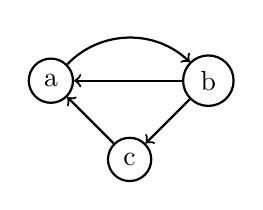
\begin{tikzpicture}[node distance={25mm}, thick, main/.style = {draw, circle}] 
        \node[main] (1) at (0,1) {a}; 
        \node[main] (2) at (2,1) {b}; 
        \node[main] (3) at (1,0) {c};  
        \draw[->] (1) edge [bend left=45] (2); 
        \draw[->] (2) -- (1); 
        \draw[->] (3) -- (1);
        \draw[->] (2) -- (3);
    \end{tikzpicture} 
    \caption{dependency graph of program in \cref{ex:dependency graph}}
    \label{fig:dependency graph}
\end{figure}


\begin{comment}
- Basic introduction to asp giving all the relevant definitions (with examples + sources (for all/some?)) 
    
    -  is  Herbrand Universe/Base needed? -> not really but should it be taken out?

-> adjust these so they work for variables etc. or do this later? (is this needed?/ is it a big adjustment?)
\end{comment}

\section{Testing in Answer Set Programming}
\label{sec:Preliminaries on answer set programming/Testing in Answer Set Programming}
In order to talk about testing answer set programs, some additional notions need to be established. Conventional testing generally consists of using a specific input to a program and observing whether the output of the program matches the expected output~\cite[71\psqq]{AO16}.

In ASP it is common practice that a problem is split in two separate programs: a \emph{problem instance} that contains the specific description of one instance of the problem class, represented as a set of facts and a \emph{uniform problem encoding} that describes the general problem class and its solutions. Thus when inputting a problem instance into the problem encoding it will find the corresponding solution and output it in form of answer sets that are usually filtered to dedicated output atoms. It is therefore natural to equate the problem instance to the conventional input and the answer sets encoding the solution to the conventional output. Based on this, we can define the \emph{input alphabet} as well as the \emph{output alphabet} of a program as a subsets of the alphabet $A$: \(\mathbb{I}_P \subseteq A\ \text{and}\ \mathbb{O}_P \subseteq A\), where the input alphabet contains all the atoms that may occur in a problem instance and the output alphabet contains the atoms relevant for the output.

In conventional software testing, a test case for a program $P$ always consists of an input $I$ of $P$ as well as the expected output of $P$ given $I$~\cite{ISO29119-1}. That way it can be verified, that a program produces the correct output given the input $I$. For an answer set program we therefore define a test case as a pair \((I, O)\) where $I$ is a set of atoms \(I \subseteq \mathbb{I}_P\) represented as facts in a input program and \(O \subseteq \mathbb{O}_P\) represents the expected output of $P$ given the input $I$ projected on the output atoms.

A \emph{test suite} for $P$ is a collection of individual test cases and the \emph{exhaustive test suite} for $P$ is the suite \(\varepsilon_P\) that contains every possible test case for $P$, meaning that for every possible input \(I \subseteq \mathbb{I}_P\) there is a test case in the exhaustive test suite that consists of $I$ and the corresponding output. There are a total of \(2^{|\mathbb{I}_P|}\) test cases in the exhaustive test suite and the inputs of $\varepsilon_P$ are the power set of the input alphabet \(inp(\varepsilon_P) = 2^{\mathbb{I}_P}\).

\begin{example}
\label{ex:test suite}
    Consider the program $P$
    \begin{align*}
        d &\leftarrow a,\ \text{not}\ b \\
        e &\leftarrow b, c \\
        f &\leftarrow a, b,\ \text{not}\ c \\
    \end{align*}
    Assuming that \(\mathbb{I}_P = \{a, b, c\}\) and \(\mathbb{O}_P = \{d, e, f\}\) a possible test case could be the pair \((I, O)\) where \(I = \{a, b\}\) and \(O = \{f\}\).
    The exhaustive test suite for this program would contain \(2^3 = 8\) different test cases: \(T_1 = (\emptyset, \emptyset)\), \(T_2 = (\{a\}, \{d\})\), \(T_3 
 = (\{b\}, \emptyset)\), \(T_4 = (\{c\}, \emptyset)\), \(T_5 = (\{a, b\}, \{f\})\), \(T_6 = (\{a, c\}, \{d\})\), \(T_7 = (\{b, c\}, \{e\})\), \(T_8 = (\{a, b, c\}, \{e\})\)
\end{example}

\begin{comment}
- maybe Specification -> the correct (expected) output for every input, what does it mean for a program to "pass/be compliant 
with" a testcase, when is a program "correct" with respect to a specification (not actually needed for coverage as coverage 
does not care about specification!)    
\end{comment}


%%%%%%%%%%%%%%%%%%%%%%%%%%%%%%%%%%%%%%%%%%%%%%%%%%%%%%%%%%%%%%%%%
\chapter{Coverage metrics}
\label{ch:Coverage metrics}
Coverage metrics in conventional software testing are a method of \emph{structural testing}, also known as \emph{white box testing}. The Idea behind white box testing is to examine a programs logic and derive test cases based this information. Therefore, this approach requires explicit knowledge of the internal structure of the program. The more parts of a programs logic (source code) are executed during a test, the more likely it is, that a bug is found. This is where coverage metrics come into play as they measure how much of a program is \emph{covered} - i.e., executed - by a test case.

There are several ways to measure this and thus, many different coverage metrics exist. Most of them take the control flow graph of a program as the basis of analysis. The most complete coverage metric is called \emph{path coverage} and measures how many of the possible paths through the control flow graph of the program are explored by a test case. The problem with this is, that the number of paths is exponential in the number of branching statements in the program and therefore this coverage metric is very expensive. A less expensive alternative in conventional testing that approximates path coverage is called \emph{branch coverage}. This entails executing each branch direction at least once, i.e., covering each edge in the control flow graph at least once~\cite[41\psqq]{MB12}.

While no real equivalent to the control flow graph exists in answer set programming, the coverage metrics that we define can be seen as the counterparts to path and branch coverage in conventional testing.

It is worth noting that due to its focus on the structure of a program, it is impossible to find errors relating to the specification of the program when using white-box testing - be it a faulty specification or the program not adhering to the specification.


\section{Coverage functions}
\label{sec:Coverage metrics/Coverage functions}
Simply speaking, the coverage of a test case is defined as the number of elements covered by the input of the test case relative to the total number of (coverable) elements. This general definition allows us to define a function schema, that can be used as the basis for different coverage metrics for different coverable elements (like programs, rules, loops etc.). 

For a class $X$ of elements the function \(\text{covered}_X(I, P)\) describes the number of elements of $X$ that are covered by some input $I$ for the program $P$. It follows that \(\text{covered}_X(2^{\mathbb{I}_P}, P)\) describes the maximum number of elements of $X$ in $P$ that can be covered by inputs from the input alphabet \(\mathbb{I}\). It is important to note that this number is often different from the total number of elements of $X$ that exist in $P$. Based on this function we introduce the \emph{basic coverage function schema} analogous to  \textcite{Jan+10} as follows:
\begin{equation}
\label{eq:coverage function schema}
    C_X(I, P) = 
    \begin{cases}
        \frac{\text{covered}_X(I, P)}{\text{covered}_X(2^{\mathbb{I}_P}, P)}, & \text{if covered}_X(2^{\mathbb{I}_P}, P) > 0 \\
        1, & \text{otherwise.}
    \end{cases}
\end{equation}

This function is standardized between 0 and 1 with worse coverage leading to a lower score. We say a collection of inputs \(I \subseteq 2^{\mathbb{I}_P}\) for program $P$ yields \emph{total coverage} with respect to a class $X$ of elements exactly if the coverage function $C_X(I, P) = 1$.

In the following we will use this schema to define a total of 5 different coverage metrics. For some of these we introduce the notions positive and negative $X$ coverage. Total $X$ coverage holds if and only if both total positive and total negative $X$ coverage hold.

\begin{comment}
    - general definition of coverage functions (maybe additional source? / compare to what paper did)   \/

    - (trivial/clairvoyant coverage functions)
\end{comment}

\section{Path-like coverage}
\label{sec:Coverage metrics/Path-like coverage}
As described above, path coverage in conventional testing is about covering every possible path through the control flow graph of the program. It is the most complete coverage metric in conventional testing, meaning that it includes any other coverage metric~\cite{Nta88}. It would therefore be the most ideal coverage metric if one were to disregard the cost of computing this metric. In practice, path coverage is almost never used. If the program contains loops that can be executed arbitrarily often, the number of possible paths becomes infinite and finding total path coverage goes from being very computationally expensive to actually impossible. 

We define here the metric \emph{program coverage} following \textcite{Jan+10}, that is analogous to conventional path coverage in that it is the most complete coverage metric for answer set programs and it is also very expensive - often unreasonably so. However a clear difference to conventional path coverage is that the maximum coverable elements can only become infinite if the program itself is infinite, as it is dependent on the number of rules in the program.


\subsection{Program coverage}
\label{subsec:Coverage metrics/Path-like coverage/Program coverage}
The idea behind program coverage is to partition the program $P$ into \emph{subprograms} \(P' \subseteq P\) and measuring how many of the possible subprograms are covered by a test case.

\begin{definition}
\label{def:program coverage}
    Let $P$ be a program, \(P' \subseteq P\) a subprogram of $P$ and $I$ an input for $P$. We say $I$ \emph{covers} $P'$ iff there is an answer set \(X \in \AS(P \cup I)\) such that \(P' = \SuppR(P, X)\).
    % \[
        % I\ \text{covers}\ P' \Longleftrightarrow \exists X \in \AS(P \cup I)\ \text{such that}\ P' = \SuppR(P, X)
    % \]
\end{definition}

We can thus define \(\text{covered}_P(I, P)\) for a collection of inputs $I$ for program $P$ as the amount of subprograms of $P$ that are covered by the inputs in $I$ and consequently instantiate the basic coverage function schema defined in \cref{sec:Coverage metrics/Coverage functions} to define \(C_P(I, P)\) the \emph{program coverage of I for P}.

\begin{example}
\label{ex:program coverage}
    Consider the program given in \cref{ex:test suite}. The input \(I = \{a, b\}\) has only one answer set: \(\AS(P \cup I) = \{\{a, b, f\}\}\). The supported rules of this answer set are: \(\SuppR(P, X) = \{f \leftarrow a, b,\ \text{not}\ c\}\) so the given input only covers a single subprogram of $P$. The total amount of subprograms that exist is \(2^{|P|} = 2^3 = 8\), however to calculate the program coverage of $I$ for $P$ we need to first calculate the number of coverable subprograms: \(\text{covered}_P(2^{\mathbb{I}_P},P) = \text{covered}_P(\{\emptyset, \{a\}, \{b\}, \{c\}, \{a, b\}, \{b, c\}, \{a, c\}, \\ \{a, b, c\}\},P) = |\ \{\emptyset, \{d \leftarrow a,\ \text{not}\ b\}, \{f \leftarrow a, b,\ \text{not}\ c\}, \{e \leftarrow b, c\}\}\ | = 4\). One can see that only half of the existing subprograms are actually coverable and thus \(C_P(I, P) = 0.25\).
\end{example}

This notion of program coverage can be very expensive to calculate as, similar to paths in a graph, the number of subprograms is exponential in the number of rules in a program. However, it is also a very powerful metric that subsumes all other coverage metrics that we will define for answer set programs. This is clear due to the fact that total program coverage of a test suite $S$ for a program $P$ implies, that every obtainable answer set of $P$ can be obtained by using only the inputs in $S$, i.e., 
\(
    \text{for inp}(S) \subseteq \mathbb{I}_P,\ C_P(\inp(S),P) = 1 \Longleftrightarrow \forall I \in \mathbb{I}_P, \forall X \in \AS(P \cup I), \exists T \in S: \exists Y \in \AS(P \cup \inp(T)) : X - \mathbb{I}_P = Y - \mathbb{I}_P
\).

% This is shown by \textcite[in theorem 2]{Jan+10}. BUT IT IS WRONG???


\begin{comment}
    - Analogous to the conventional path-like coverage I define program coverage    \/
    
    - Definition + example      \/
    
    - show that total program coverage means all possible answer sets get produced by the testsuite
    
    - talk about the problems here? (complexity + not possible for programs with variables as it is necessary to enumerate all 
    possible inputs to find maximum coverage)
\end{comment}

\section{Branch-like coverage}
\label{sec:Coverage metrics/Branch-like coverage}
Since in conventional testing, path coverage is often not realistically achievable, many more metrics have been developed that intend to approximate path coverage while keeping the cost much lower. They generally consist of defining some subset of all paths that needs to be covered. Depending on the size of this subset the metric can be more or less powerful and more or less expensive. One of the most widely used metrics that approximate path coverage is branch coverage, also known as edge coverage. It consists of covering each direction after a branching statement at least once. This is equivalent to requiring each edge of the control flow graph to be covered at least once~\cite[Chapter 7.2]{AO16}.

In the following, we use the definitions given by \textcite{Jan+10} to introduce four different coverage metrics that, like branch coverage in conventional testing, try to approximate the path-like metric of program coverage while being simpler to compute.

\begin{comment}
    - general introduction to branch-like coverage in conventional programming languages (source)     \/
    
        - use the control flow graph and cover every possible branch through this graph   \/
    
    - less complete but easier to compute, still very potent(?) (source)    (\/)
    
    - there are different types of branch like coverage even in conventional programming languages (source), the same is true here      \/

    - maybe example for both branch and path coverage?? -> requires conventional program as example -> maybe not
\end{comment}

\subsection{Rule coverage}
\label{subsec:Coverage metrics/Branch-like coverage/Rule coverage}
We start by introducing the simplest one of the branch-like metrics called \emph{rule coverage}. Here, the focus is on the rules of a program, which means the coverage of a test case $T$ is decided by checking whether each individual rule in the program $P$ is supporting or not for each answer set \(X \in \AS(P \cup \inp(T))\).

\begin{definition}
\label{def:rule coverage}
    Let $P$ be a program and $I$ an input for $P$. A rule \(r \in P\) is \emph{positively rule covered} by $I$ iff there is an answer set \(X \in \AS(P \cup I)\) such that \(X \models B(r)\), i.e., the rule is supported by the answer set.
    % \[
        % I\ \text{positively covers}\ r \in P \Longleftrightarrow \exists X \in \AS(P \cup I)\ \text{such that}\ X \models B(r)
    % \]
    On the other hand, a rule $r$ is \emph{negatively rule covered} by $I$ iff there is some answer set $X$ such that \(X \not\models B(r)\)
    % \[
        % I\ \text{negatively covers}\ r \in P \Longleftrightarrow \exists X \in \AS(P \cup I)\ \text{such that}\ X \not\models B(r)
    % \]
\end{definition}

For a collection of inputs $I$ for a program $P$ we define \(\text{covered}_{R^+}(I, P)\) and \(\text{covered}_{R^-}\\(I, P)\) as the number of rules that are positively (respectively negatively) covered by an input in $I$, and again, the basic coverage function schema~(\ref{eq:coverage function schema}) is used to define \(C_{R^+}(I, P)\ \text{and}\ C_{R^-}(I, P)\) as the \emph{positive and negative rule coverage} of $I$ for $P$. We call \(C_R(I, P)\) the \emph{rule coverage} of $I$ for $P$ based on the function \(\text{covered}_{R}(I, P) = \text{covered}_{R^+}(I, P) + \text{covered}_{R^-}(I, P)\).

\begin{example}
\label{ex:rule coverage}
    We again look at the program from \cref{ex:test suite} with two different inputs \(I_1 = \{a, b\}\) and \(I_2 = \{b, c\}\). The corresponding answer sets are \(\AS(P \cup I_1) = \{\{a, b, f\}\} = \{X_1\}\) and \(\AS(P \cup I_2) = \{\{b, c, e\}\} = \{X_2\}\). Therefore the first input covers the third rule of the program positively, as \(X_1 \models B(r_3)\) holds, and the two other rules negatively, while the second input covers the second rule positively (\(X_2 \models B(r_2)\)) and the first and third rule negatively. Considering all 3 rules can be both positively and negatively covered, a test suite $S$ containing these two inputs would yield a positive rule coverage of \(C_{R^+}(S, P) = 2/3\), a negative rule coverage of \(C_{R^-}(S, P) = 1\) and a rule coverage of \(C_R(S, P) = 5/6\).
\end{example}

Analogous to how some subprograms may not be coverable by any input (see \cref{ex:program coverage}), it is also possible for rules to not be positively or negatively coverable. For example a fact can never be negatively covered, as any interpretation will always satisfy an empty body. On the other hand, rules of the form "\(a \leftarrow \text{not}\ a.\)" can never be positively covered. This is due to the fact that any interpretation that satisfies the body of this rule can not be an answer set of the program containing this rule.

\begin{example}
\label{ex:special rules}
    Consider the program \(P = \{a \leftarrow \text{ not } a\}\).
    The interpretation \(I = \emptyset\) satisfies the body or the rule (\(I \models B(r)\)) since \(B^+(r) = \emptyset \subseteq I\) and \(B^-(r) = \{a\} \cap I = \emptyset\) both hold. However $I$ does not satisfy the rule, because while \(I \models B(r)\) holds, \(I \cap H(r) \neq \emptyset\) does not hold. Therefore $I$ is not a model for this program and no model can exists that satisfies the body of this rule.
\end{example}

Consequently, this also means that constraints can never be positively rule covered. This is obvious when considering that a constraint "\(\leftarrow a.\)" is nothing other than a shorthand notation for the rule "\(x \leftarrow a, \text{ not } x.\)", where $x$ is a new atom, which matches the pattern of the rule in \cref{ex:special rules} \cite[p. 17]{Geb+12}. It is also possible for a normal rule to not be positively or negatively coverable due to the program surrounding it, for example if an atom that is never defined in the program and not part of the input alphabet occurs positively in the body of a rule, this rule can never be positively covered. Note however that any rule has to always be either positively or negatively covered.

Finally it is easy to see that rule coverage is indeed implied by program coverage, as rule coverage only considers the coverage of each rule individually, while program coverage looks at all possible sets of rules. As an example a program with a total of four rules has 16 coverable elements for program coverage only four of which are coverable elements for rule coverage.

\begin{comment}
    - Definition + example      \/
    
    - (similar to program coverage in some ways but less complex!)
    
    - some rules may sometimes (or always) not be coverable -> examples -> ties back to beginning of the chapter / thats why coverage 
    is defined on coverable objects     \/
    
    (- total program coverage implies total rule coverage -> not so relevant but maybe interesting to mention?)      \/
\end{comment}

% \subsubsection{Constraint coverage}
% \label{subsubsec:Coverage metrics/Branch-like coverage/Rule coverage/Constraint coverage}
% [SHOULD I DEFINE THIS??] Probably not here - maybe next chapter

\begin{comment}
    - constraints are a special type of rule and have to be handled slightly differently because when the body of a constraint is true 
    (=normal rule coverage) this will imply false and therefore not create an answer set / create an unsatisfiable solve call -> we 
    cant check constraints the same way we check other rules
    
    - solution: (following the suggestion in the paper by \textcite{Jan+11}) remove the constraint from the program in order to check 
    for its covereage!
    
    - Definition + examples
    
    (- maybe reminder that these coverage metrics dont really care about what the output of the program is and whether its according to 
    the specification, therefore removing constraints is okay even though it might completely destroy the functionality of the program)
\end{comment}

\subsection{Loop coverage}
\label{subsec:Coverage metrics/Branch-like coverage/Loop coverage}
Since rule coverage only considers individual rules, it can not explore possible connections between rules or atoms. On the other hand, a concept that has been shown to be very important when computing answer sets is the concept of loops in answer set programs \cite{LZ04}. Therefore, a matching coverage metric is also introduced to capture these positive dependencies between atoms in the program.

\begin{definition}
\label{def:loop coverage}
    Let $P$ be a program and $I$ an input for $P$. A loop $L$ of $P$ is \emph{positively loop covered} by $I$ iff there is some answer set \(X \in \AS(P \cup I)\) such that for every atom \(a \in L\) there is a rule \(r \in \SuppR(P, X)\) with \(r \in \Def(a)\), i.e., every atom in the loop can be derived from the program and its input.
    % \[
        % I\ \text{positively covers}\ L :\Longleftrightarrow \exists X \in\ \AS(P \cup I)\ \forall a \in L\ \exists r \in \Def(a): r \in \SuppR(P,X)
    % \]
    The loop $L$ is \emph{negatively loop covered} by $I$ iff there is some answer set $X$ such that for at least one atom \(a \in L\) for which \(\Def(a) \neq \emptyset\) holds, no rule \(r \in \SuppR(P, X)\) exists with \(r \in \Def(a)\).
    % \begin{align*}
        % I\ \text{negatively covers}\ &L :\Longleftrightarrow \exists X \in\ \AS(P \cup I):\ \exists a \in L\ \text{for which}\ \Def(a) \neq \emptyset \\ 
        % &\text{and}\ \nexists r \in \Def(a)\ \text{for which}\ r \in \SuppR(P,X)
    % \end{align*}
\end{definition}

As above, we again define for program $P$ and the input collection $I$ for $P$ \(C_{L^+}(I, P)\), \(C_{L^-}(I, P)\) and \(C_{L}(I, P)\) as the (\emph{positive} or \emph{negative}) \emph{loop coverage} of $I$ for $P$.

Since positive (resp. negative) loop coverage for $L$ requires, that for every (resp. at least one) atom \(a \in L\), \(\Def(a) \neq \emptyset\) holds, loops containing atoms that only appear in the body of rules can not be positively (negatively) covered. Although this can only happen with singleton loops, because in order for an atom $a$ to be part of a loop of size two or more, it needs to have at least one incoming edge in the positive atom dependency graph, thus \(| \Def(a) | \geq 1\).

\begin{example}
\label{ex:loop coverage}
    Consider the program $P$
    \begin{align*}
        a &\leftarrow b, c \\
        b &\leftarrow a, d \\
        a &\leftarrow e,\ \text{not}\ c
    \end{align*}
    with \(\mathbb{I}_P = \{a, b, c, d, e\}\). We can achieve total rule coverage for $P$ with the three test inputs \(I_1 = \{b, c\}\), \(I_2 = \{a, d\}\) and \(I_3 = \{e\}\). However, while these inputs cover the two singleton loops \(\{a\}\) and \(\{b\}\) positively and negatively, the loop \(L = \{a, b\}\) between the first two rules is only negatively covered. In order to positively cover $L$, a different input such as \(I_4 = \{b, c, d\}\) is needed.
    Note that inputs \(I_1, I_2\) and \(I_4\) together yield total loop coverage, as the singleton loops \(\{c\}\), \(\{d\}\) and \(\{e\}\) can not be positively loop covered.
\end{example}

The problem with loop coverage is that the number of loops in a program is, in the worst case, exponential in the number of rules of the program. Thus, while it is still an approximation of program coverage, i.e., total program coverage implies total loop coverage~\cite{Jan+10}, it can be a rather expensive metric to compute. Therefore the next two coverage metrics are introduced to approximate loop coverage.

\begin{comment}
    - loops play an important role in ASP as seen in (source). Therefore constructing a coverage metric that focuses on them makes sense        \/
    
    - Definition + example      \/
    
    - generally number of loops in a program in exponential in the number of rules -> expensive to compute! -> introduce 2 more coverage metrics that approximate loop coverage! (one for minimal (singleton) loops and one for maximal loops (strongyl connected components))      \/
    
    (- no real relation to rule coverage (neither implies the other)
    
    - total program coverage implies total loop coverage -> not so relevant but maybe interesting to mention?)
\end{comment}

\subsection{Definition coverage}
\label{subsec:Coverage metrics/Branch-like coverage/Definition coverage}
There are two ways to think about the definition coverage metric. On one hand, it is, as mentioned above, an approximation of loop coverage as it simply looks at only the coverage of the singleton loops of a program. On the other hand one could say that definition coverage is a metric that looks at the \emph{definable atoms} of a program $P$, i.e., the set of atoms $a_i$ for which \(\Def(a_i) \neq \emptyset\) holds, as opposed to rule coverage looking at rules.

\begin{definition}
\label{def:definition coverage}
    Let $P$ be a program, $I$ an input for $P$ and $A$ the set of definable atoms of $P$. An atom \(a \in A\) is \emph{positively definition covered} by $I$ iff there is an answer set \(X \in \AS(P \cup I)\) such that there is a rule \(r \in \SuppR(P, X)\) with \(r \in \Def(a)\), i.e., the atom can be derived from the program and its input.
    % \[
    %     I \text{ positively covers } a \in A \Longleftrightarrow \exists X \in \AS(P \cup I) \text{ such that } \exists r \in \Def(a), r \in \SuppR(P, X)
    % \]
    The atom $a$ is \emph{negatively definition covered} by $I$ iff there is an answer set $X$ such that there is no rule \(r \in \SuppR(P, X)\) for which \(r \in \Def(a)\) holds.
    % \[
    %     I \text{ negatively covers } a \in A \Longleftrightarrow \exists X \in \AS(P \cup I) \text{ such that } \nexists r \in \Def(a), r \in \SuppR(P, X)
    % \]
\end{definition}

We define \(C_{D^+}(I, P)\) and \(C_{D^-}(I, P)\) as the \emph{positive} and \emph{negative definition coverage} for an input collection $I$ and a program $P$, as well as the \emph{definition coverage} \(C_D(I, P)\), in the same way as with the other metrics.

It is important to note that total positive rule coverage implies total positive definition coverage but total negative rule coverage does not imply total negative definition coverage. However, since definition coverage is effectively singleton loop coverage, total loop coverage implies total definition coverage.

\begin{example}
\label{ex:definition coverage}
    Consider the program and inputs from \cref{ex:loop coverage}. Inputs $I_1$, $I_2$ and $I_3$ together yield total rule coverage as well as total definition coverage since both singleton loops \(\{a\}\) and \(\{b\}\) are both positively and negatively covered. It is however also possible to achieve total definition coverage with just the two inputs $I_1$ and $I_2$ or $I_2$ and $I_3$. On the other hand while the two inputs \(I_1 = \{b, c\}\) and \(I_5 = \{a, d, e\}\) yield total rule coverage, they do not negatively definition cover the atom $a$ and thus only yield total positive definition coverage.
\end{example}

Whether or not an atom is (positively or negatively) coverable always depends on the rules of the program it appears in. An atom appearing as a fact in a program will always be positively definition covered and thus can not be negatively definition covered.

\begin{comment}
    - 2 ways to introduce definition coverage:  \/
        
        - as a coverage metric for singleton loops (minimal loops) and therefore a special case of loop coverage        \/
    
        - as a representation of the disjunctions in the program (if an atom "a" is defined in multiple rules you could rewrite this as a if B1 v B2 v ...) -> this coverage metric covers these implicit disjunctions
    -> discuss both but in which order?     \/
    
    - Definition + example      \/
    
    (- this is different to rule coverage! -> total positive rule coverage implies total positive definition coverage, not the other way around and no connection for negative coverage!       \/
    
    - total loop coverage implies total definition coverage     \/
    
    - total program coverage implies total definition coverage)
\end{comment}

\subsection{Component coverage}
\label{subsec:Coverage cetrics/Branch-like coverage/Component coverage}
As seen above, definition coverage is a metric pertaining to the minimal loops of a program. Component coverage on the other hand is focused on the maximal loops of a program, i.e., its strongly connected components. As such it functions similarly to loop coverage with only a small difference in the definition of negative coverage.

\begin{definition}
\label{def:component coverage}
    Let $P$ be a program and $I$ an input for $P$. A strongly connected component $C$ of $P$ is \emph{positively component covered} by $I$ iff there is an answer set \(X \in \AS(P \cup I)\) such that for every atom \(a \in C\) there is a rule \(r \in \SuppR(P, X)\) with \(r \in \Def(a)\).
    % \[
    %     I \text{ positively covers } C \Longleftrightarrow \exists X \in\ \AS(P \cup I) \text{ such that } \forall a \in C,\ \exists r \in \Def(a), r \in \SuppR(P,X)
    % \]
    The component $C$ is \emph{negatively component covered} by $I$ iff there is an answer set \(X \in \AS(P \cup I)\) such that for every atom \(a \in C, \Def(a) \neq \emptyset\) holds and there is no rule \(r \in \SuppR(P, X)\) with \(r \in \Def(a)\).
    % \begin{align*}
    %     I \text{ negatively covers } C \Longleftrightarrow &\exists X \in\ \AS(P \cup I) \text{ such that } \forall a \in C,\ \Def(a) \neq \emptyset \text{ and } \\
    %     &\exists r \in \Def(a), r \in \SuppR(P,X)
    % \end{align*}
\end{definition}

Once more the (\emph{positive} or \emph{negative}) \emph{component coverage} for an input collection $I$ and a program $P$ is defined using the schema \ref{eq:coverage function schema}, yielding \(C_{C^+}(I, P)\), \(C_{C^+}(I, P)\) and \(C_{C}(I, P)\).

As with all the branch-like metrics, component coverage is implied by program coverage and just like definition coverage, it is an approximation of loop coverage and thus total positive loop coverage implies total positive component coverage.
Because negative component coverage is defined slightly different than negative loop coverage (none of the atoms in the SCC can be supported as opposed to just one atom being unsupported is enough) negative component coverage is not implied by negative loop coverage, however it does allow the following result: if a component $C$ is positively (negatively) component covered, all loops that are contained in this component \(L \subseteq C\) are also positively (negatively) loop covered \cite[Theorem 7]{Jan+10}.

\begin{example}
\label{ex:component coverage}
    Consider again the program and inputs from \cref{ex:loop coverage}. The input \(I_4 = \{b, c, d\}\) yields total positive component coverage as the only coverable component is the SCC \(C = \{a, b\}\). In order to achieve total negative component coverage, none of the rules of the program can be supported. Thus an input such as \(I = \emptyset\) works. Notice how the input $I$ also negatively covers the two singleton loops \(\{a\}\) and \(\{b\}\) that are contained in the SCC.
\end{example}

Now we have introduced two different coverage metrics that successfully approximate loop coverage in that they are significantly less expensive to compute while still trying to capture the essence of what loop coverage is about. Especially when used together, definition and component coverage come relatively close to the functionality of loop coverage, however for both metrics the number of coverable elements is always capped by the number of rules in the program. This is because in a propositional program, only one atom can be defined per rule and there can only be at maximum as many coverable SCCs as there are definable atoms. This means that both these metrics are significantly easier to compute that loop coverage.


\begin{comment}
    - strongly connected components are the maximal loops of the program, therefore this is an approximation of loop coverage       \/  
    
    - Definition + example      \/
    
    - Definition of negative coverage is different from loop coverage! \/
    
    - because of this different definition positive/negative component coverage of a specific component implies positive/negative loop 
    coverage for all subset loops of the component (would not be the case for negative coverage if definition is different)     \/
    
    (- total positive loop coverage implies total positive component coverage, however this is not true for negative coverage because 
    of the different definition (see above)     \/
    
    - total program coverage implies total component coverage)  \/

    (- with the help of definition coverage one could redefine loop and component coverage based on definition coverage)

    - both definition coverage and component coverage are capped on the number of rules in the program      \/
\end{comment}

%%%%%%%%%%%%%%%%%%%%%%%%%%%%%%%%%%%%%%%%%%%%%%%%%%%%%%%%%%%%%%%%%
\chapter{Computing coverage metrics for propositional programs}
\label{ch:Computing coverage metrics for propositional programs}
One of the main contributions of this thesis is finding a way to implement the coverage metrics defined in the previous chapter and building a prototype tool for checking coverage of answer set programs. Since the definitions in their current form are only for propositional programs the implementation is also focused on that. However there is very little real world use for a coverage tool that can only work with propositional programs as almost no real world answer set program is exclusively propositional. Therefore it would be beneficial to choose an approach that can be easily extended to incorporate more complex programs. The attempt for such an extension is made in the next chapter.

\begin{comment}
    - one of the main contributions of this thesis is finding a way to build a prototype tool for checking coverage of ASP programs based on the theoretic definitions of coverage described in the previous chapter.   \/
    
    - as the definitions are only applicable to propositional programs, those will be my focus for now. However such a tool would not be very practical so ideally an approach should be chosen that can easily be extended.    \/
    
    (maybe include a short history of what i tried but didnt work? -> meta programming with reify output)
\end{comment}

\section{General approach}
\label{sec:Computing coverage metrics for propositional programs/General approach}
The goal of this approach is to find a way to compute the different coverage metrics defined in the previous chapter using the power of ASP itself. In order to achieve this, we introduce a syntactic transformation of the original program. 

The idea of the transformation is to add new rules to the program containing special \emph{label atoms} for every coverage metric and every coverable element. These label atoms have to be atoms that are not contained in the original alphabet $A$ of the program. Afterwards the program can be ground and solved normally and the coverage can be calculated by checking which label atoms are contained in the answer set. Since the rules that are added to the program can only produce label atoms that are not used anywhere else in the program and no existing rules are changed, the result of the transformation is still semantically equivalent to the original program. Another advantage of this approach is, that it is not necessary to compute every model of the program. Instead it is sufficient to only compute the brave and cautious consequences which is much more efficient.

The same idea of adding label atoms can also be used in order to add the test inputs to the program. This allows us to compute the total coverage of all inputs contained in a test suite in the same solve call instead of using separate solve calls for each test input. However, according to the basic coverage functions schema, in order to calculate the coverage we need not only the elements covered by the test input but also the maximum coverable elements. This can easily be done in the same way by using a test input containing a choice rule of all atoms in the input alphabet $\mathbb{I}_P$. 

\begin{comment}
    - the goal is to compute the coverage using ASP     \/
    
    -> introduce labels for each coverage metric -> add them to the program in a specific way (based on the coverage metric)  -> solve normally using clingo -> if the label is in the answer set, the corresponding object is covered      \/
    
    - I only add new rules, dont change or take away existing ones (except constraints -> see above) and these new rules only produce labels not predicates that are part of the original program -> the resulting program is still equivalent! (maybe proof?)      \/
    
    - with this method, to find total positive and negative coverage it is not necessary to look at every model in the solve call. Instead use one solve call with brave consequences and one with cautious consequences! -> more efficient than looking at every model!        \/
    
    - labels can also be used to add the testcases to the program -> this way coverage for all testcases can be computed in the same solve call instead of needing one call per testcase        \/
    
    -> this is done by: adding a choice rule $\{\_i0;...;\_in\}$. for n testcases in the testsuite, adding rules $a_i :- i_j$. for every atom i in the testcase j.
    (- why does this work?
    - why does this not change the program?)
    
    - maximum coverage needs to be computed to get accurate coverage numbers!       \/
    
    -> done by calculating the coverage normally but instead of testcases adding a rule $\{a_0;...;a_n\}$. where $a_0...a_n$ are all possible inputatoms (see definition input/output) -> these have to be specified in advance by the user!
\end{comment}

\section{Test input}
\label{sec:Computing coverage metrics for propositional programs/Test input}
First we will take a better look at how the test inputs of the test suite are added to the original program using the syntactic transformation. As mentioned in \cref{sec:Preliminaries on answer set programming/Testing in Answer Set Programming}, a test suite can contain multiple test cases and each test case contains one test input represented as a set of atoms. The transformation is done by adding a choice rule to the program, containing label atoms for each test case in a test suite. This choice rule represents "choosing" one of the test cases and additional rules will then add all the atoms contained in the chosen test input to the program.

\begin{definition}
\label{def:input transforamtion}
    Let $P$ be a program and $S$ a test suite containing test cases \(T_1, \ldots, T_n\). The input of each test case $T_i$ is a set of input atoms \(\inp(T_i) = \{a_1, \ldots,a_m\}\). The \emph{input transformation} is defined as follows:
    \begin{enumerate}
        \item Add a choice rule to program $P$: \(\{\_i_0; \ldots;\_i_n\} = 1.\) where each $\_i_i$ is a label atom associated with the input of test case $T_i$
        \item For every test case \( T_j \in S\) and for every atom \( a_i \in \inp(T_j)\) add a rule to $P$: \(a_i \leftarrow \_i_j.\) where $\_i_j$ is the label atom corresponding to test case $T_j$
    \end{enumerate}
\end{definition} 

When the test suite contains only one test case, the result of this transformation will be the same as concatenating the original program with the test input - minus the label atoms which do not change the behavior of the program. On the other hand when the test suite contains multiple test cases, the results of all test cases can be calculated with just one solve call thanks to this transformation.

\begin{example}
\label{ex:input transformation}
    Consider the simple program $P$
    \begin{align*}
        c &\leftarrow a \\
        d &\leftarrow b
    \end{align*}
    and the test suite \(S = \{T_1, T_2\}\) where \(\inp(T_1) = \{a\}\) and \(\inp(T_2) = \{b\}\). When using the input transformation to add $S$ to $P$, rules will be added according to the definition above and the transformed program $P'$ will look like this:
    \begin{align*}
        c &\leftarrow a \\
        d &\leftarrow b \\
        \{\_i_1; \_i_2\} = 1 &\leftarrow \\
        a &\leftarrow \_i_1 \\
        b &\leftarrow \_i_2
    \end{align*}
    the resulting answer sets are \(\AS(P') = \{\{\_i_1, a, c\}, \{\_i_2, b, d\}\}\) thus yielding the same answer sets - not counting label atoms - as adding the two inputs separately to the program, i.e., \(\AS(P \cup \inp(T_1)) = \{\{a, c\}\}\) and \(\AS(P \cup \inp(T_2)) = \{\{b, d\}\}\).
\end{example}

\section{Rule coverage}
\label{sec:Computing coverage metrics for propositional programs/Rule coverage}
Next we will look at the syntactic transformation used to compute rule coverage for a program $P$. In order to check the coverage of each rule we will introduce label atoms for each rule by adding new rules such that whenever the label atom for rule $i$ is in an answer set, the rule is positively covered and when the label is not in the answer set it is negatively covered. This way in order to calculate the rule coverage one can simply count the rule label atoms in the answer sets.

As seen in \cref{subsec:Coverage metrics/Branch-like coverage/Rule coverage}, a rule is positively rule covered if the body of the rule is satisfied and otherwise it is negatively covered. We add the rule labels according to this definition.

\begin{definition}
\label{def:rule transformation}
    Let $P$ be a program containing rules \(r_1, \ldots, r_n\). The \emph{rule coverage transformation} works as follows:
    \begin{itemize}
        \item for every rule \(r_i \in P\) add a rule to $P$: \(\_r_i \leftarrow B(r_i).\) where each $\_r_i$ is a label atom associated with the rule $r_i$
    \end{itemize}
\end{definition}

This translation guarantees a correct calculation of the positive and negative rule coverage by simply counting the rule label atoms in the produced answer sets. Specifically, computing the brave consequences of the augmented program $P$ for an input $I$ will yield every rule label atom that has been derived in at least one answer set of $P$. The positive rule coverage of $I$ for $P$ can therefore be calculated by counting these label atoms. However in this case we can not simply count the missing label atoms to calculate the negative rule coverage because that way we would only count the rules that are only negatively and not positively covered by the input. To get the full negative coverage we have to first compute the cautious consequences, which will only contain the label atoms for those rules, that are only positively covered and not negatively covered. Now counting the missing labels will yield the negative rule coverage of $I$ for $P$.

\begin{proof}
    Given a program $P$ which has been transformed using the rule coverage transformation and an interpretation $I$, assume $I$ positively covers a rule \(r_i \in P\). Then there is an answer set \(X \in \AS(P \cup I)\) such that \(X \models B(r_i)\). This means that the rule \(\_r_i \leftarrow B(r_i).\) is supported and thus the label atom $\_r_i$ has to be in the answer set $X$. In the same way, assume there is an answer set \((X \in \AS(P \cup I)\) such that \(\_r_i \in X\). This is only possible if the rule \(\_r_i \leftarrow B(r_i).\) is supported, i.e., \(X \models B(r_i)\). Therefore, according to the definition, the rule $r_i$ is positively rule covered by $I$. The proof for negative coverage looks the same.
\end{proof}

\begin{example}
\label{ex:rule transformation}
    Consider the program $P$ and the test suite $S$ from \cref{ex:input transformation}. 
    When using the rule transformation to prepare the program for a rule coverage check, two new rules will be added to $P$:
    \begin{align*}
        \_r_1 &\leftarrow a \\
        \_r_2 &\leftarrow b 
    \end{align*}
    if we then add the test suite to the program using the input translation like before and solve the program normally the following answer sets are produced \(\AS(P') = \{\{\_i_1, a, c, \_r_1\}, \{\_i_2, b, d, \_r_2\}\}\). We notice that the first answer set only contains the label for the first rule and the second contains only that of the second rule. This means the first test input positively covers the first rule and negatively covers the second rule and the second test input does the opposite and thus the entire test suite yields total rule coverage. It is easily verified that this is the correct result.
\end{example}

\begin{comment}
- $\_ri$ label for every rule i     \/

- add new rule to program for each label: $\{\_ri\}$ is the head, the body is identical to the body of the rule i       \/

- example           \/

- if the body of rule i is true in some answer set (aka $X |= B(r_i)$) then rule i is positively covered and $\_ri$ will appear in the answer set       \/

-> $\_ri$ in answer set <=> rule i is positively covered        \/

-> $\_ri$ not in answer set <=> rule i is negatively covered (proof for these?) \/
\end{comment}

\section{Definition coverage}
\label{sec:Computing coverage metrics for propositional programs/Definition coverage}
From here on, the following transformations will each be based on a previous transformation. The transformation used to compute definition coverage in particular is based on the rule coverage transformation. This keeps each individual transformation very simple and straight forward. Because of this, the following transformations do not need to directly interact with the original program and only work off of the previously introduced label atoms. The disadvantage is that sometimes a transformation has to be made even if the corresponding coverage metric will not be computed. 

As a reminder, definition coverage checks, whether at least one of the defining rules of an atom is supported by a program under an interpretation. Checking whether a rule is supported is already done by the rule coverage transformation, so we can use the rule label atoms to derive new definition label atoms.

\begin{definition}
\label{def:definition transformation}
    Let $P$ be a program containing rules \(r_1, \ldots, r_n\), $A$ its alphabet and $A_D$ the set of definable atoms of $P$ (\(A_D = \{a \in A\ |\ \Def(a) \neq \emptyset\}\)). The \emph{definition coverage transformation} works as follows:
    \begin{itemize}
        \item For every definable atom \(a_i \in A_D\) and for every rule \(r_j \in \Def(a_i)\) add a rule to $P$: \(\_d_i \leftarrow \_r_j.\) where $\_r_j$ is the label atom for rule $r_j$ and each $\_d_i$ is a new label atom associated with the atom $a_i$
    \end{itemize}
\end{definition}

It is important to note that the alphabet $A$ of program $P$ is that of the original program and thus does not contain any label atoms. Therefore already introduced label atoms will not create additional rules during the definition coverage transformation and will thus not affect the coverage calculation.
As mentioned, this transformation only requires the label atoms derived from the rule coverage translation and is able to correctly represent the definition coverage metric so that whenever a label $\_d_i$ is in an answer set the corresponding atom is positively definition covered. For those label atoms that are not in the answer set one has to distinguish between the definable atoms and those that are not definable. Only the definable atoms that do not have a label in an answer set count as negatively definition covered. This also works with brave and cautious consequences in the same way as the rule coverage transformation.

\begin{proof}
    Given a program $P$ which has been transformed using both the rule and the definition coverage transformation and an interpretation $I$, assume $I$ positively covers an atom $a_i$. Then there is an answer set \(X \in \AS(P \cup I)\) such that there is a rule \(r_j \in \SuppR(P, X)\), meaning that $r_j$ is positively rule covered and thus $\_r_j \in X$ holds, with \(r_j \in \Def(a_i)\), meaning that there is a rule \(\_d_i \leftarrow \_r_j.\). Since \(\_r_j \in X\) holds, $\_d_i$ has to also be in the answer set.

    Given a program $P$ which has been transformed using both the rule and the definition coverage transformation and an interpretation $I$, assume $I$ positively (negatively) covers atom $a_i$ but the associated label atom $\_d_i$ is not in any answer set (is contained in an answer set) \(X \in \AS(P \cup I)\). According to the definition of definition coverage, there is a \(X \in \AS(P \cup I)\) such that there is a (no) rule \(r_j \in \SuppR(P, X)\) with \(r_j \in \Def(a_i)\). Because rule $r_j$ defines atom $a_i$ the transformation added a rule \(\_d_i \leftarrow \_r_j.\) and since $r_j$ is (not) supported, the atom $\_r_j$ has to (not) be in the answer set and thus $\_d_i$ has to (not) be in $X$ which contradicts the assumption.
    
    % \(I \text{ positively definition covers } a_i \in A \Longleftrightarrow 
    % \exists X \in \AS(P \cup I) \text{ such that } \exists r_j \in \Def(a_i), r_j \in \SuppR(P, X) \Longleftrightarrow 
    % \exists r_j \in \Def(a_i), \_r_j \in X \Longleftrightarrow
    % \_d_i \in X \in \AS(P \cup I)\) and
    % \(I \text{ negatively definition covers } a_i \in A \Longleftrightarrow 
    % \exists X \in \AS(P \cup I) \text{ such that } \not\exists r_j \in \Def(a_i), r_j \in \SuppR(P, X) \Longleftrightarrow 
    % \not\exists r_j \in \Def(a_i), \_r_j \in X \Longleftrightarrow
    % \_d_i \not\in X \in \AS(P \cup I)\)
\end{proof}

\begin{example}
\label{ex:definition transformation}
    Consider again the program $P$ and test suite $S$ from \cref{ex:input transformation}. We again use the rule coverage transformation as described in \cref{ex:rule transformation}. If we now add the definition coverage transformation there will again be two new rules added, as the program $P$ only contains two definable atoms which are each only defined once in the program. Assuming that the atom $c$ will be associated with the label atom $\_d_1$ and the atom $d$ with $\_d_2$, the added rules will look like this:
    \begin{align*}
        \_d_1 &\leftarrow \_r_1 \\
        \_d_2 &\leftarrow \_r_2
    \end{align*}
    In this trivial case the definition coverage is identical to the rule coverage, as any input that achieves total rule coverage will also achieve total definition coverage and vice verse, so it is easy to see that the transformation is correct in this case. However if we add a third rule to the original program such as \(d \leftarrow a.\), running both transformations will yield the program $P'$:
    \begin{align*}
        c &\leftarrow a      &  \_r_1 &\leftarrow a      &  \_d_1 &\leftarrow \_r_1 \\
        d &\leftarrow b      &  \_r_2 &\leftarrow b      &  \_d_2 &\leftarrow \_r_2 \\
        d &\leftarrow a      &  \_r_3 &\leftarrow a      &  \_d_2 &\leftarrow \_r_3 
    \end{align*}
    In this example we can see that the same atom can be covered by two different rules which is reflected by having two rules with the same label atom in the head.
\end{example}

Note that in the example above, even though there are no label atoms in any answer set that correspond to the atoms $a$ and $b$, they do not count as negatively definition covered because they are not definable. This is why it is not sufficient to look which labels are missing in an answer set when calculating negative definition coverage. 

\begin{comment}
    - $\_di$ label for every atom i     \/
    
    - if atom i is definable (it appears in the head of a rule, aka $Def(a_i)\neq\emptyset$) add new rule to program: $\_di :- \_rj$. for every rule j that defines atom i 
    (every rule j that has atom i in its head, aka every $r_j \in Def(a_i)$)    \/
    
    - example           \/
    
    - if one of the rules is covered (its body is true) then atom i is covered and $\_di$ will appear in the answer set     \/
    
    -> $\_di$ in answer set <=> atom i is positively covered    \/
    
    -> $\_di$ not in answer set <=> atom i is negatively covered (proof for these?)  \/
\end{comment}

\section{Loop coverage}
\label{sec:Computing coverage metrics for propositional programs/Loop coverage}
The loop coverage transformation is based on the previously introduced transformation for definition coverage. This is an obvious choice, as the basis of loop coverage is the same as that of definition coverage, namely checking whether specific atoms are defined in a program. The only difference with loop coverage is, that all atoms in a loop have to be defined in the same answer set. This makes the actual transformation again rather simple. 

The problem with loop coverage is, that in order to find the loop coverage one needs to first find the loops of the program. To do that, we need to build the positive atom dependency graph of the program and then find all loops in the resulting graph. Only once all loops are found, the following transformation can be done.

\begin{definition}
\label{def:loop transformation}
     Let $P$ be a program and $L$ the set of all loops of $P$. The \emph{loop coverage transformation} works as follows:
    \begin{itemize}
        \item For every loop \(l_i \in L\), \(l_i = \{a_1, a_2, \ldots, a_n\}\) add a rule to $P$: \(\_l_i \leftarrow \_d_1, \_d_2, \ldots, \_d_n.\) where $\_l_i$ is a new label atom associated with the loop $l_i$ and each $\_d_i$ is the label for atom $a_i$.
    \end{itemize}
\end{definition}

Once again, this transformation only uses previously introduced label atoms and does not interact in any way with the original program. Also thanks to this translation we can once again calculate the loop coverage simply based on if the label for a specific loop is in an answer set or not.

\begin{proof}

\end{proof}

\begin{example}
\label{ex:loop transformation}
    Consider the program from \cref{ex:loop coverage}. This program has a total of six loops (five singleton loops and the loop $\{a, b\}$) therefore the loop coverage transformation will add six new rules to the program:
    \begin{align*}
        \_l_1 &\leftarrow \_d_1  &  \_l_2 &\leftarrow \_d_2  &  \_l_3 &\leftarrow \_d_3 \\
        \_l_4 &\leftarrow \_d_4  &  \_l_5 &\leftarrow \_d_5  &  \_l_6 &\leftarrow \_d_1, \_d_2 
    \end{align*}
    Note that the atoms $c$, $d$ and $e$ never appear in the head of a rule in $P$, thus they are not definable and their corresponding label atoms $\_d_3$, $\_d_4$ and $\_d_5$ can never be derived. This means that the label atoms for the corresponding singleton loops can also never be derived which is the expected behaviour as these loops can never be positively covered.
\end{example}

\begin{comment}
- $\_li$ label for every loop i     \/

- first need to find all the loops in the program! -> build positive atom dependency graph, find sccs and then find subsets of sccs that are loops  \/

- for each loop i that consists of atoms $a_m$ to $a_n$ add new rule to program: $\_li :- \_dm, ..., \_dn$.     \/

- if all the atoms $a_m$ to $a_n$ that constitute the loop i are defined (aka definition covered), then all the $\_dm$ to $\_dn$ are true, then loop i is covered and $\_li$ will be in the answer set.     \/

-> $\_li$ in answer set <=> loop i is positively covered

- if any of the atoms $a_m$ to $a_n$ are not defined the loop is negatively covered and  $\_li$ will not be in the answer set       \/

-> $\_li$ not in answer set <=> loop i is negatively covered
\end{comment}

\section{Component coverage}
\label{sec:Computing coverage metrics for propositional programs/Component coverage}
The definition for the component coverage metric is very similar to that of loop coverage and this is reflected also in the transformation. However, component coverage is the only metric where something not being positively covered does not necessarily mean that it is negatively covered. Because of this, we will need to add two new label atoms for each strongly connected component - one to calculate positive coverage and one for negative coverage - instead of just one. Additionally, as with the loop coverage transformation, it is necessary to first find all the SCCs of the program.

\begin{definition}
\label{def:component transformation}
    Let $P$ be a program and $C$ the set of all strongly connected components of $P$. The \emph{component coverage transformation} works as follows:
    \begin{itemize}
        \item For every SCC \(s_i \in C\), \(s_i = \{a_1, a_2, \ldots, a_n\}\) add two rules to $P$:
        \begin{itemize}
            \item \(\_s_i \leftarrow \_d_1, \_d_2, \ldots, \_d_n.\) where $\_s_i$ is a new label atom associated with the SCC $s_i$ and each $\_d_i$ is the label for atom $a_i$.
            \item \(\_ns_i \leftarrow \text{not } \_d_1, \text{not } \_d_2, \ldots, \text{not } \_d_n.\) where $\_ns_i$ is a new label atom associated with the SCC $s_i$ and each $\_d_i$ is the label for atom $a_i$.
        \end{itemize}
    \end{itemize}
\end{definition}

Using this transformation, it is possible to calculate the positive component coverage by counting the $\_s_i$ label atoms and the negative component coverage by checking the $\_ns_i$ labels. Because of the additional labels for negative coverage, it is possible to calculate both positive and negative coverage by just computing the brave consequences of the program. This method guarantees correctness according to the definition of the metric.

\begin{proof}
    
\end{proof}

\begin{example}
\label{ex:component transformation}
    Consider again the program from \cref{ex:loop coverage}. The program has four strongly connected components thus the component coverage transformation will add a total of eight rules to the program:
    \begin{align*}
        \_s_1 &\leftarrow \_d_1, \_d_2  &  \_ns_1 &\leftarrow \text{not } \_d_1, \text{not } \_d_2 \\
        \_s_2 &\leftarrow \_d_3  &  \_ns_2 &\leftarrow \text{not } \_d_3 \\
        \_s_3 &\leftarrow \_d_4  &  \_ns_3 &\leftarrow \text{not } \_d_4 \\
        \_s_4 &\leftarrow \_d_5  &  \_ns_4 &\leftarrow \text{not } \_d_5 
    \end{align*}
    The last six rules are about the atoms $c$, $d$ and $e$ that are not definable. Here it is clear to see that the corresponding singleton loops - which are also SCCs - are always negatively covered and the labels $\_ns_2$, $\_ns_3$ and $\_ns_4$ will be contained in every answer set.
\end{example}

\begin{comment}
- $\_si$ label for every strongly connected component i

- find sccs same way as loops

- construct new rules same way as for loops: $\_si :- \_dm, ... , \_dn$.

-> $\_si$ in answer set <=> scc i is positively covered

- HOWEVER! $\_si$ not in answer set -/> scc i is negatively covered! (see definition of component coverage)

-> add additional rules to program: $\_nsi :- not \_dm, ..., not \_dn$.

- if NONE of the atoms $a_m$ to $a_n$ are defined (aka definition covered), scc i is negatively covered and $\_nsi$ will be in the anser set

-> $\_nsi$ in answer set <=> scc i is negatively covered
\end{comment}

\section{Program coverage}
\label{sec:Computing coverage metrics for propositional programs/Program coverage}
The final coverage metric that needs to be discussed is program coverage. As a reminder, program coverage looks at subprograms of the main program. These subprograms are again just sets of rules that need to be supported. This means we can base the program coverage transformation on the rule coverage transformation, since that transformation is used to check if a rule is supported. The big difference for program coverage is, that it checks whether entire sets of rules are supported in the same answer set. 

There are two different ways to compute the program coverage. The first is to use the rule label atoms derived in each answer set to 

\begin{comment}
- use the $\_ri$ labels from rule coverage, no new labels needed!

- a subprogram $P' \subseteq P$ is covered if exactly all rules contained in $P'$ are covered and no other rules are covered

- two ways to go about computing it!

-> each answer set covers exactly one subprogram -> it is necessary to look at every answer set instead of just brave/cautious like 
with the other coverage metrics -> has to be computed seperately from the other coverage metrics!

- for $P = \{r_1,...,r_n\}$,  $\{\_rx,...,\_ry\}$ are the rule labels in an answer set <=> $P'=\{r_x,...,r_y\}$ is covered
\end{comment}

\section{Implementation details}
\label{sec:Computing coverage metrics for propositional programs/Implementation details}
In this section we will take a brief look at an implementation of the above transformations. I build a prototype tool for checking coverage for answer set programs that applies the defined semantic transformations and uses the power of ASP to calculate all five coverage metrics for any propositional normal logic program. The implementation is done using the integrated ASP system \emph{clingo} [SOURCE] and it's python API. 

In order to implement the transformations and use them to calculate coverage there are three main steps. First, information on the program needs to be gathered. This includes for example gathering the atoms that appear in the program and finding which of them are definable. Second, new rules are added to the original program based on the information that has been gathered and the defined transformations. Finally, the modified program is solved using the clingo solver and the coverage is calculated from the computed brave and cautious consequences.

\subsection{Information gathering}
\label{subsec:Computing coverage metrics for propositional programs/Implementation details/Information gathering}
The information gathering is done using the \emph{abstract syntax tree} (AST) of the program. This is a representation of a non-ground program that can be generated using the clingo.ast module of the clingo python API [SOURCE]. It contains all the necessary information about the rules in the program and the atoms in the head and the body of each rule. 

The \code{parse\_files} function is used to parse the original program statement by statement and pass each statement as an abstract syntax tree to the \code{gather\_info} function. This function will analyze each AST node and save all relevant info in an appropriate data structure. The main one is a dictionary that uses atom names and arity as the keys and saves the location of the atom in the original program, a unique label associated with that atom and the labels of all the rules that define the atom in the values. The latter two make it easy to later construct the rules for the definition coverage transformation, the location is only used to allow for a better output. Additionally, the AST nodes containing an entire rule are saved in a list. This list is later used during the rule coverage transformation for easy access to the bodies of each rule. It is also used to build the positive atom dependency graph of the program and for printing results.

\begin{example}
\label{ex:information gathering}
    Consider the simple program $P$:
    \begin{align*}
        c &\leftarrow a \\
        d &\leftarrow b
    \end{align*}
    the corresponding abstract syntax tree can be seen in \cref{fig:ast example}. The atom dictionary for this program will look like this after information gathering:
    
    \code{atoms = \{(c, 0): [[0], [location], [0]], (d, 0): [[1], [location], [1]], (a, 0): [[2], [location], []], (b, 0): [[3], [location], []]\}}

    Where the first value is the atom label and the third value is the label of the rule it is defined in. Atoms $a$ and $b$ have an empty list as last value since they are not defined in this program.
\end{example}

\begin{figure}[h]
    \centering
    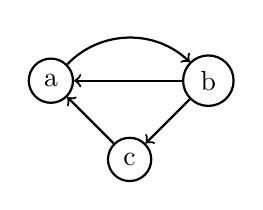
\begin{tikzpicture}[node distance={25mm}, thick, main/.style = {draw, circle}] 
        \node[main] (1) at (0,1) {a}; 
        \node[main] (2) at (2,1) {b}; 
        \node[main] (3) at (1,0) {c};  
        \draw[->] (1) edge [bend left=45] (2); 
        \draw[->] (2) -- (1); 
        \draw[->] (3) -- (1);
        \draw[->] (2) -- (3);
    \end{tikzpicture} 
    \caption{abstract syntax tree of program in \cref{ex:information gathering}}
    \label{fig:ast example}
\end{figure}

It is obvious even from this small example that the abstract syntax tree carries way more information than we require. Thus some work has to be done to make sure that the correct information is gathered for every possible type of AST node. This also takes into account all the additional language constructs that exist in the input language for clingo.

What is also done in the \code{gather\_info} function is removing \code{\#show} statements from the original program. This is done because show statements can interfere with the calculation of coverage. Since they have no impact on the functionality of the program, removing them is not a problem. This is done at this specific point because here each AST node of the original program is analyzed anyways. Thus it is simple to remove each show statement by replacing it with a simple \code{\#true} statement that has no impact on the program whatsoever.

Since the information gathered in this function is relevant for each coverage metric, this function is always executed, no matter which metric will be computed. Another part of the information gathering is building the positive atom dependency graph of the program and finding all its loop and strongly connected components. This is done by going through every rule of the program and adding nodes and edges one by one to the graph using the networkX package. Then, the \code{strongly\_connected\_components} method of networkX is used to find all the SCCs in the constructed graph. Finally the remaining loops that are not SCCs are found by going through the power set of each SCC and checking, whether each set is strongly connected or not. Especially building the dependency graph this way is not very efficient but this only needs to be done if loop or component coverage will be computed and can be skipped otherwise.

\subsection{Adding rules}
\label{subsec:Computing coverage metrics for propositional programs/Implementation details/Adding rules}
There are multiple ways how one can add new rules to an non-ground program using the clingo python API. In this case, the rules are build using functions from the AST module of clingo and the program builder class is used to add the rules to the non-ground program. 

There is a separate function for each transformation. That way it is possible to only perform the transformations that are required. Each of these functions works very similarly. Thanks to the work done during information gathering, data structures already exist that contain everything needed for each transformation. All that is left to do is go through the appropriate structure for each transformation, build the rules accordingly and use a program builder to add them to the program.

As an example you can see the function used for the loop coverage transformation in \cref{lst:find_loops}. It uses the set \code{self.loops}, which is a set of tuples. Each tuple represents on loop of the program and contains the keys (name and arity) for every atom in the loop.

\begin{lstlisting}[float,caption={Function implementing the loop coverage transformation},label=lst:find_loops]
def add_loops(self):
    with ProgramBuilder(self.ctl) as bld:
        for idx, loop in enumerate(self.loops):
            body = []
            pos = ast.Position('<string>', 1, 1)
            loc = ast.Location(pos, pos)
            fun = ast.Function(loc, '_l{}'.format(idx), [], False)
            atm = ast.SymbolicAtom(fun)
            head = ast.Literal(loc, ast.Sign.NoSign, atm)
            for key in loop:
                fun = ast.Function(loc, '_d{}'.format(self.heads[key][0][0]), [], False)
                atm = ast.SymbolicAtom(fun)
                lit = ast.Literal(loc, ast.Sign.NoSign, atm)
                body.append(lit)
            bld.add(ast.Rule(loc, head, body))
            # print(ast.Rule(loc, head, body))

\end{lstlisting}

\subsection{Calculating coverage}
\label{subsec:Computing coverage metrics for propositional programs/Implementation details/Calculating coverage}
Once all rules are added, the program is ground and then solved twice. Once using the brave modeling and once using cautious modeling...

\begin{comment}
show in general terms:
- how i am using the AST of the program to gather information about rules and (definable) atoms
    - what information is gathered? why? how is it stored?

- how i am using ProgramBuilders to add new rules to the program using the gathered information (obviously only add what is necessary based on which metric should be computed)
    - how are the rules added? how do i know which rules to add?

- how i read the label atoms from the answer sets and use them to calculate the coverage (plus printing information about covered / not covered elements is possible)
    - how is the program solved? (brave/cautious using clingo...) how do i gather the resulting models/the contained atoms? how do i compute coverage from the gathered atoms?
\end{comment}

%%%%%%%%%%%%%%%%%%%%%%%%%%%%%%%%%%%%%%%%%%%%%%%%%%%%%%%%%%%%%%%%%%%%%%%%%%%%%%%%%%%%%%
\chapter{Coverage for further program classes}
\label{ch:Coverage for further program classes}


\begin{comment}
- the given definitions of the coverage metrics are only for propositional programs but this is not very practical as most programs 
are more complex than that. They contain many complex language constructs supported by ASP/clingo

-> to make this coverage check actually usable these metrics have to be extended to work for all these constructs

- in general, the label approach should allow me to easily apply these coverage metrics to further program classes with very little 
adjustments!
\end{comment}

\section{Adjusted definitions}
\label{sec:Coverage for further program classes/Adjusted definitions}


\begin{comment}
- starting with basic definitions, which have to be changed? -> list here

- then go through coverage metric definitions -> if they dont have to be changed, why?
\end{comment}

\section{Language constructs}
\label{sec:Coverage for further program classes/Language constructs}


\begin{comment}
- go through all the additional constructs one by one, explain how they should work, why they do work like that or not?
-> table

- Big difference: maximal coverage can not be computed as this requires listing all possible inputs. This is not possible with variables 
as there can be infinitely many -> give coverage as covered/total existing (!!! is this even a correct coverage function???)
(!!! possible extension: allow user to specify domain for each variable -> if domain is not infinite then computing max cov is possible !!!) 

-> thats all the difference!?!
\end{comment}

%%%%%%%%%%%%%%%%%%%%%%%%%%%%%%%%%%%%%%%%%%%%%%%%%%%%%%%%%%%%%%%%%%%%%%%%%%
% \chapter{Implementation}
% \label{ch:Implementation}

% \section{Adjusted definitions}
% \label{sec:Coverage for further program classes/Adjusted definitions}

% \section{Adjusted definitions}
% \label{sec:Coverage for further program classes/Adjusted definitions}
%%%%%%%%%%%%%%%%%%%%%%%%%%%%%%%%%%%%%%%%%%%%%%%%%%%%%%%%%%%%%%%%%%%%%%%%%%
\chapter{Conclusion}
\label{ch:Conclusion}


\begin{comment}
(Zusammenfassung)
- I managed to implement the coverage metrics defined by \textcite{Jan+10} in a way that makes it possible to compute the coverage of an entire test suite with the help of just 2 clingo solve calls

- I also extended the coverage metrics to cover almost all existing language constructs in ASP/clingo, making them more "real world" applicable


(Outlook)
- As mentioned in the previous section, theory atoms and constraint terms are currently not considered when calculating definition, loop and component coverage -> should be an easy extension!

- rebuilding the app to work with the ClingoApp could make working with external atoms, constants and different program parts possible or easier (by allowing interaction with the clingo solver through the command line)

- in this work, complexity and efficiency are not priorities, therefore the current program is not very optimized!

- for this prototype I tried to take the existing definitions of coverage in ASP and extend them to more complex programs with as little changes to the definitions as possible. This might not be the best way! Some of the definitions might need more changes:

    - Definition coverage and choice rules: if an atom is only defined in a choice rule (ex. $\{a\}.$) it will only be considered positively     covered, not negatively covered, if the body is true, even though the atom will be false in some answer sets (therefore acting as if it was negatively covered -> the "path" where the atom is negatively covered is executed, but the atom is not considered negatively covered)

    - loop/component coverage: a loop is considered covered, if all atoms contained in the loop are definition covered. Due to the nature of definition coverage it is however possible for an atom to be covered at multiple places! -> it is thus possible to cover all atoms in a loop without ever "executing" the loop -> this can lead to problems that are caused by a loop not being discovered by a testcase, even though that testcase has total loop coverage! (example!)

- simply checking coverage for a given testsuite is only one use case for coverage metrics! They can also be used to automatically generate testcases that are meant to catch a maximum amount of errors. The idea is explored in \cite{Jan+11}. This can certainly also be done with my implementation.

- these coverage metrics have not really been tested! In the paper \cite{Jan+11} only rule and definition coverage have been tested for their practicality in a "real world" scenario. It is unknown how effective loop and component coverage are. -> This needs testing! During these tests potential changes to the definitions could also be evaluated.

- also in the line of testing the coverage metrics it would be interesting to see how well definition and component coverage approximate loop coverage and whether program coverage does actually give the best results given that it is the most "complete" metric -> maybe figure out a guideline on which metrics to use when. The current setup where mixing any metrics is possible does not make much sense (as for example definition coverage is fully contained in loop coverage)!


(Fazit)
- in this thesis I laid the ground work to one day implement coverage checks and maybe coverage-based testgeneration in a full unit testing api for ASP programs

- the simple nature of my approach should make it easy to extend to program with new or improved coverage metrics and implement it into a larger testing framework

- this is working towards making Answer Set Programming more accessible and more efficient by providing tools to support the developpement process
\end{comment}


%%%%%%%%%%%%%%%%%%%%%%%%%%%%%%%%%%%%%%%%%%%%%%%%%%%%%%%%%%%%%%%%%

\chapter{Test}
\label{ch:Test}

\begin{enumerate}
    \item Bla.\\
    (Bla.)
    \item Bla. (Bla.)
\end{enumerate}

\Cref{ch:Introduction} Referenz zu Kapitel.
\Cref{sec:Test/Perzepte_und_Symbole} Referenz zu Unterkapitel. 
\Cref{fig:cups_yolo} Referenz zu Bild.
\Cref{lst:cups_symbolic} Referenz zu Listing
\textcite{Jan+10} Zitat mit Namen der Autoren
\cite{Jan+10} Zitat nur mit Abkürzung
\ac{ASP} Link zu Abkürzungen
\emph{symbol grounding problem} 
\marginpar{Symbol} Randkommentar
\footnote{Bla} Fussnote

\section{Perzepte und Symbole}
\label{sec:Test/Perzepte_und_Symbole}
Bla.

%\begin{definition}
%    \label{def:Perzept}
%    Ein \emph{Perzept}\marginpar{Perzept} ist der sensorische Eindruck eines physikalischen Objektes zu einem bestimmten Zeitpunkt.
%\end{definition}

\begin{figure}
    \centering
    \includegraphics[width=0.4\textwidth]{gfx/unilogo.jpg}
    \caption{Ein Kamerabild mit eingezeichneten Perzepten.}
    \label{fig:cups_yolo}
\end{figure}


\begin{lstlisting}[float,caption={Eine symbolische Beschreibung der Objekte in bla.},label=lst:cups_symbolic]
symbol(cup_1; cup_2; cup_3; spoon; diningtable).

is_on(
    cup_1, diningtable;
    cup_2, diningtable;
    cup_3, diningtable
).

is_inside_of(spoon, cup_3).

contains(
    cup_1, coffee;
    cup_2, coffee;
    cup_3, hot_chocolate
).

\end{lstlisting}



%\begin{figure}
%    \centering
%    \begin{tikzpicture}[
%        ->,
%        >={Stealth[round]},
%        align=center,
%        state/.style={
%            draw,
%            rectangle,
%            rounded corners=3mm
%        },
%        every edge/.append style={thick}
%    ]
%        \node (A) [state]             {Symbol verankert};
%        \node (B) [state, below=of A] {Symbol nicht verankert};
%
%        \node (1) [left =25mm of A, font=\scriptsize] {ausgehend von\\einem Perzept};
%        \node (2) [right=25mm of A, font=\scriptsize] {ausgehend von\\einem Symbol};
%        \node (3) [below=of B,      font=\scriptsize] {Symbol gelöscht};
%
%        \path (A) edge [loop above] node [above] {\emph{Verfolgen}}    (A);
%        \path (A) edge [bend left]  node [right] {\emph{Verlieren}}    (B);
%        \path (B) edge [bend left]  node [left]  {\emph{Wiederfinden}} (A);
%        \path (1) edge              node [above] {\emph{Entdecken}}    (A);
%        \path (2) edge              node [above] {\emph{Finden}}       (A);
%        \path (B) edge              node [right] {\emph{Zerstören}}    (3);
%    \end{tikzpicture}
%    \caption{Die Verankerungsfunktionen als Zustandsübergänge, frei nach \cite[Abbildung~4]{Gün+18}.}
%    \label{fig:anchoring_functions_as_state_transitions}
%\end{figure}




$$\operatorname{match}(\sigma, \gamma) \Leftrightarrow \forall p \in \sigma \; \exists \phi \in \operatorname{feat}(\gamma): \; g(p, \phi, \gamma(\phi))$$


\begin{table}
    \centering
        \begin{tabularx}{0.5\textwidth}{l|X|l}
            $M$             & $P_1^M$                               & $Cn(P_1^M)$  \\
            \hline
            $\emptyset$     & $\{ a \leftarrow a, b \leftarrow \}$  & $\{ b \}$     \\
            $\{ a \}$       & $\{ a \leftarrow a \}$                & $\emptyset$   \\
            $\{ b \}$       & $\{ a \leftarrow a, b \leftarrow \}$  & $\{ b \}$     \\
            $\{ a, b \}$    & $\{ a \leftarrow a \}$                & $\emptyset$   \\
        \end{tabularx}
    \caption[$P_1 = \{ a \leftarrow a, b \leftarrow naf a \}$ hat ein stabiles Modell.]{$P_1 = \{ a \leftarrow a, b \leftarrow naf a \}$ hat ein stabiles Modell $\{ b \}$.}
    \label{tab:Ein_stabiles_Modell}
\end{table}

%\begin{example}
%    Das Programm $P = \{ \; \{ a, b\} \; \}$ hat vier stabile Modelle, nämlich die Elemente von $2^{\{a, b\}}$.
%\end{example}

%\begin{example}
%   Das Programm
%    $$
%        P =
%        \begin{Bmatrix}
%            \operatorname{cup}(1) \\
%            \operatorname{cup}(2) \\
%            1~\{~\operatorname{blue}(X) : \operatorname{cup}(X)~\}~1 \\
%        \end{Bmatrix}
%    $$
%    hat die Grundinstanz
%    $$
%        \grd(P) =
%        \begin{Bmatrix}
%            \operatorname{cup}(1) \\
%            \operatorname{cup}(2) \\
%            1~\{~\operatorname{blue}(1),~\operatorname{blue}(2)~\}~1 \\
%        \end{Bmatrix}
%    $$
%    und die stabilen Modelle $\{\operatorname{cup}(1),{ }\operatorname{cup}(2),{ }\operatorname{blue}(1)\}$ und \linebreak$\{\operatorname{cup}(1),{ }\operatorname{cup}(2),{ }\operatorname{blue}(2)\}$.
%\end{example}

\begin{proof}
    Zu jeder Teilmenge $M \subseteq A = \{ a, b, c \}$ ist $P^M = P$.
    Die Teilmengen~$\emptyset$, $\{ a \}$, $\{ c \}$, $\{ a, b \}$ und $\{ b, c \}$ sind keine Modelle von $P^M$. $\{ a, c \}$, $\{ a, b, c\}$ und $\{ b \}$ sind Modelle von $P^M$.
    $\{ a, b, c\}$ ist kein minimales Modell von $P^M$, da $\{ b \} \subseteq \{ a, b, c\}$.
    Da $\{ a, c \} \nsubseteq \{ b \}$ und $\{ b \} \nsubseteq \{ a, c \}$, sind beide Modelle minimal und damit stabile Modelle von $P$.
\end{proof}

\code{\#show p(X,Y) : q(X).}

Test für \code{\#show p(X)} in einer Zeile.
%\lstinputlisting[float,caption={[Ein Graph mit 6 Knoten und 17 Kanten\\(\code{graph.lp}).]Ein Graph mit 6 Knoten und 17 Kanten (\code{graph.lp}).},label=lst:graphcolor/graph.lp]{../../code/graphcolor/graph.lp}

\begin{align*}
    &X                          &=\ &\{ \text{cup}_1, \text{cup}_2 \} \\
    &\Pi                        &=\ &\{ \pi_1, \pi_2, \pi_3 \} \\
    &\Phi                       &=\ &\{ \text{coffee}, \text{tea}, \text{hot}, \text{cold} \} \\
    &T                          &=\ &\{ t_1, t_2 \} \\
    &\beta(\text{cup}_1, t_1)   &=\ &\{ \text{coffee} \} \\
    &\beta(\text{cup}_2, t_1)   &=\ &\emptyset \\
    &\beta(\pi_1, t_1)          &=\ &\{ \text{coffee} \} \\
    &\beta(\pi_2, t_1)          &=\ &\{ \text{tea}, \text{cold} \} \\
    &\beta(\pi_3, t_2)          &=\ &\{ \text{tea} \}
\end{align*}


\cleardoublepage
